\section{Proceso} 

\textbf{Ejercicio 1: Crear relaciones}

\begin{itemize}
	\item En el cuadro de dialogo Explorador, seleccionar las hojas DimCurrency, DimCustomer, DimDate, DimProduct, DimPromotion, DimSalesTerritory, y FactInternetSales.
	\begin{center}
	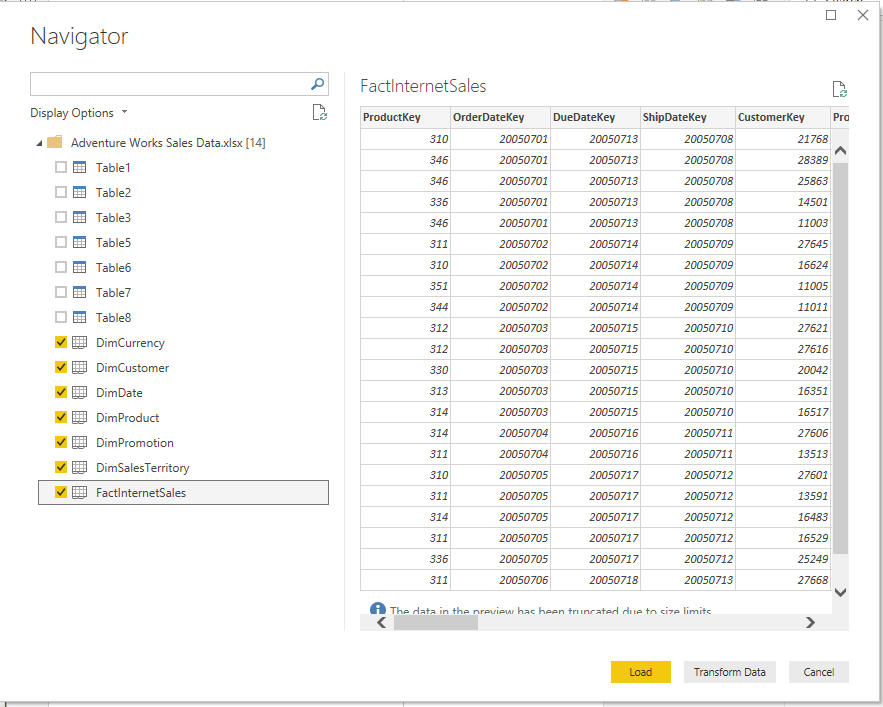
\includegraphics[width=10cm]{./Imagenes/Captura1} 
	\end{center}
\end{itemize} 

\begin{itemize}
	\item Vista Fields de las hojas seleccionadas.
	\begin{center}
	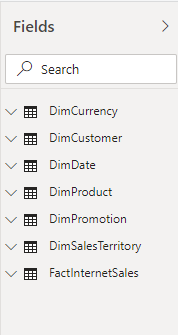
\includegraphics[width=5cm]{./Imagenes/Captura2} 
	\end{center}
\end{itemize} 

\begin{itemize}
	\item  Panel de modelamiento.
	\begin{center}
	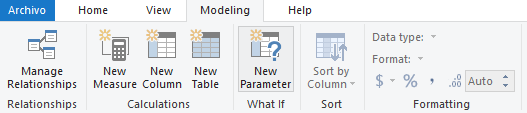
\includegraphics[width=10cm]{./Imagenes/Captura3} 
	\end{center}
\end{itemize} 

\begin{itemize}
	\item Cuadro de Administrar relaciones (Manage Relationships).
	\begin{center}
	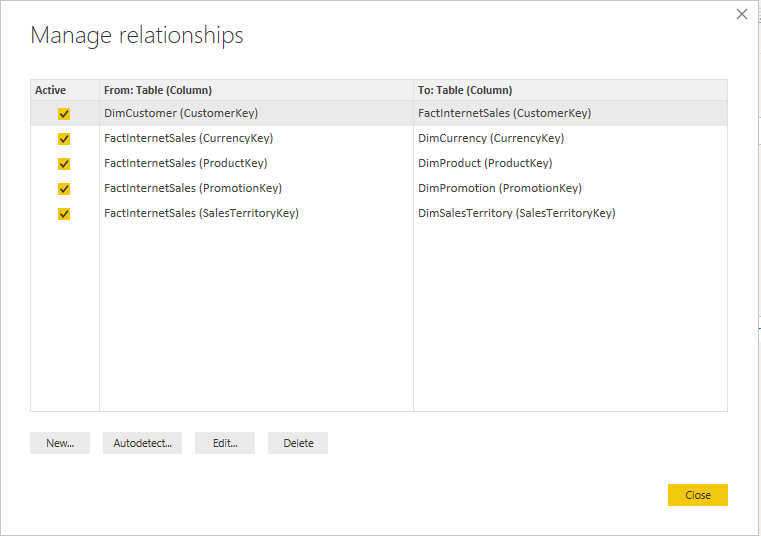
\includegraphics[width=10cm]{./Imagenes/Captura4} 
	\end{center}
\end{itemize} 

\begin{itemize}
	\item Creado una nueva relacion en el cuadro de Administrar relaciones.
	\begin{center}
	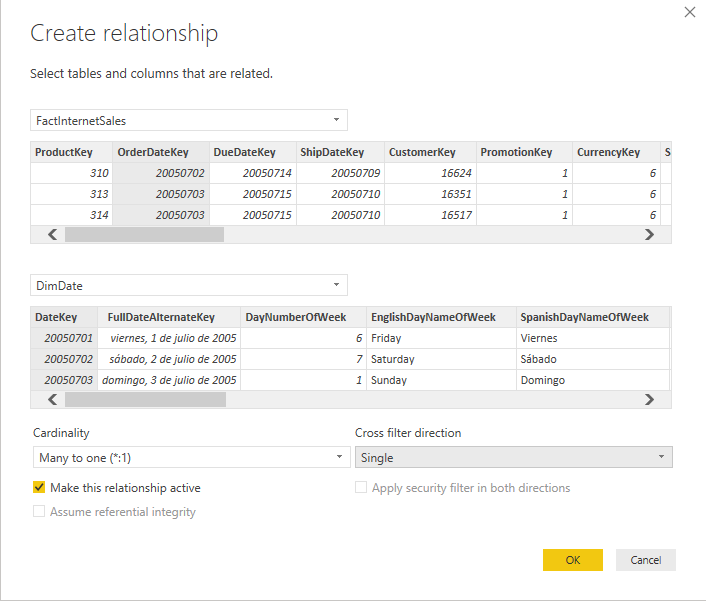
\includegraphics[width=10cm]{./Imagenes/Captura5} 
	\end{center}
\end{itemize} 

\begin{itemize}
	\item Vista de Modelo de todas las relaciones.
	\begin{center}
	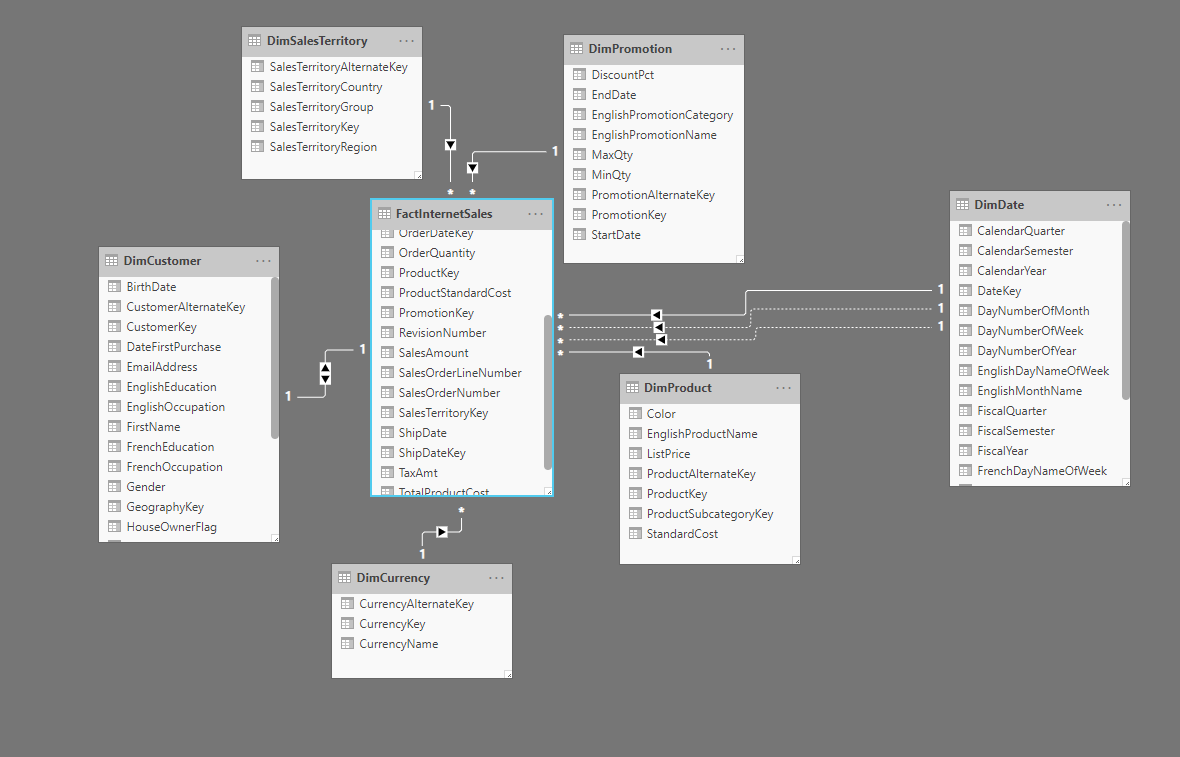
\includegraphics[width=13cm]{./Imagenes/Captura6} 
	\end{center}
\end{itemize} 

\begin{itemize}
	\item Eliminar la línea de la relación entre DimProductCategory, y DimProductSubcategory.
	\begin{center}
	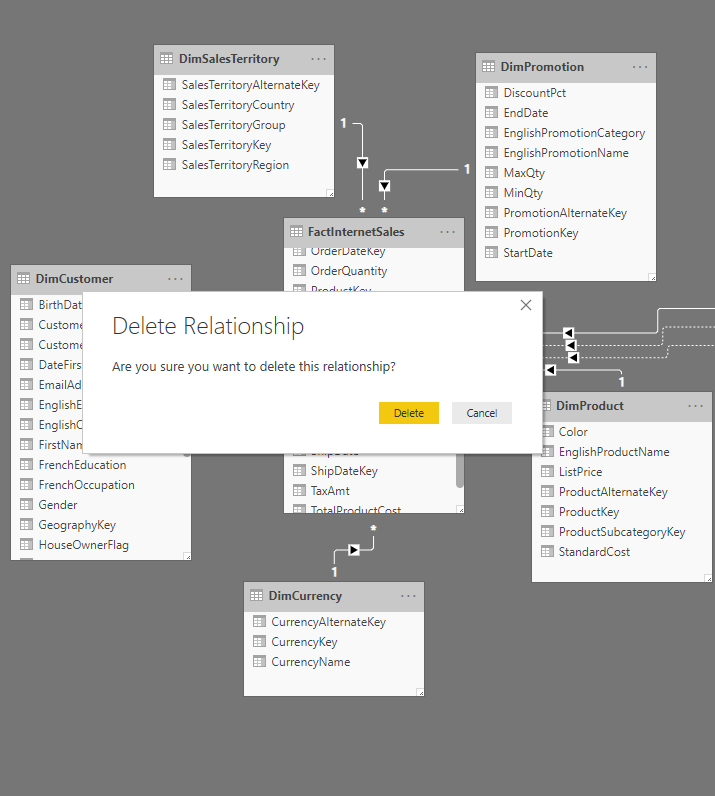
\includegraphics[width=13cm]{./Imagenes/Captura7} 
	\end{center}
\end{itemize} 
\begin{itemize}
	\item Creando una nueva relacion entre FactInternetSales y CustomerKey.
	\begin{center}
	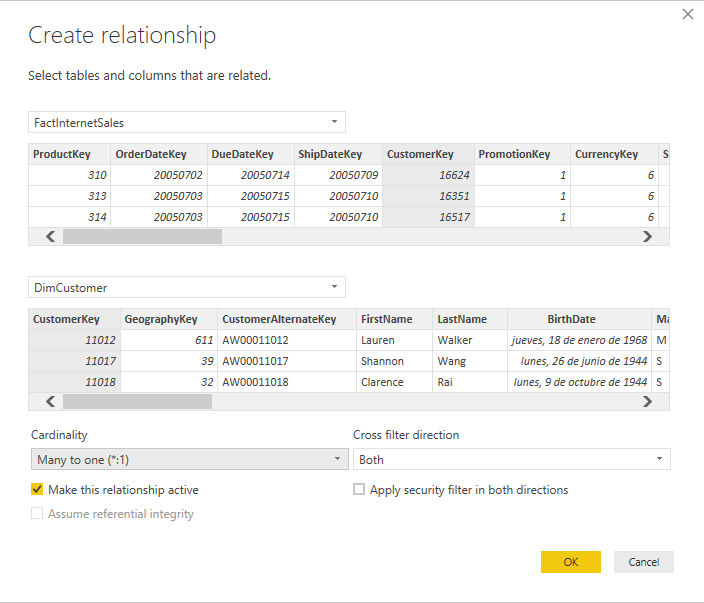
\includegraphics[width=13cm]{./Imagenes/Captura8} 
	\end{center}
\end{itemize} 


\textbf{Ejercicio 2: Relaciones manuales}


\begin{itemize}
	\item cuadro de dialogo Explorador, seleccionar las hojas DimProductCategory, y DimProductSubcategory.
	\begin{center}
	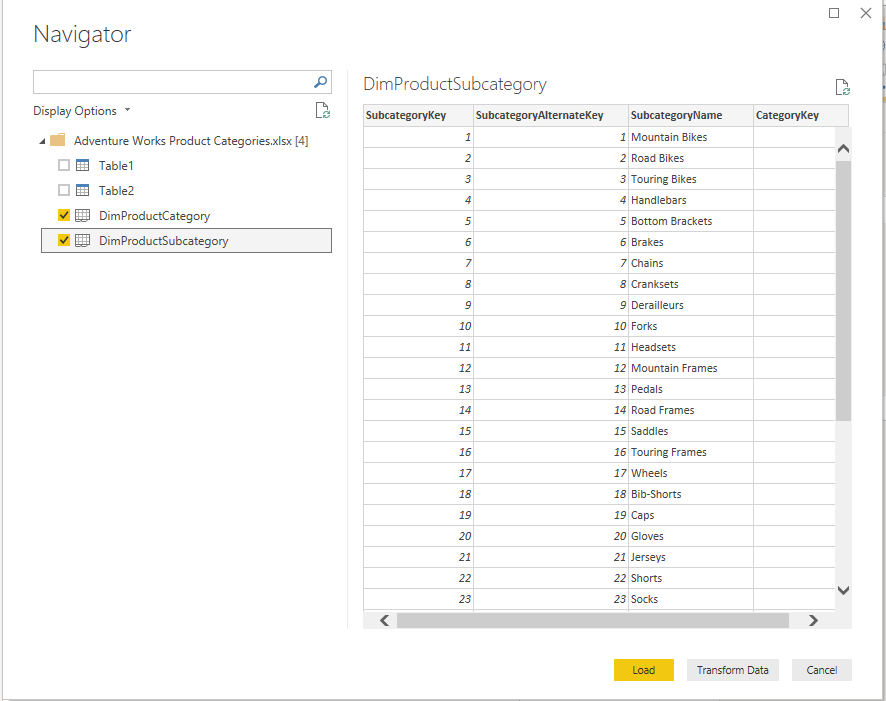
\includegraphics[width=13cm]{./Imagenes/Captura2-1} 
	\end{center}
\end{itemize} 

\begin{itemize}
	\item Vista de Modelo de la relacion.
	\begin{center}
	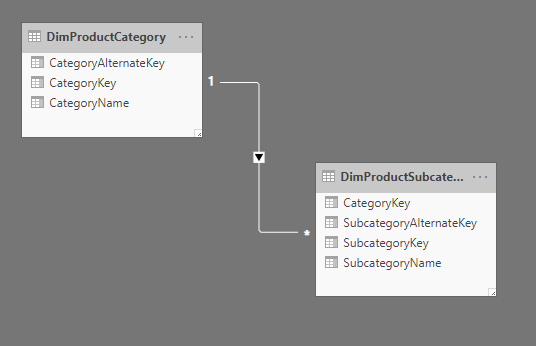
\includegraphics[width=13cm]{./Imagenes/Captura2-2} 
	\end{center}
\end{itemize} 

\begin{itemize}
	\item Eliminando la línea de la relación entre DimProductCategory, y DimProductSubcategory.
	\begin{center}
	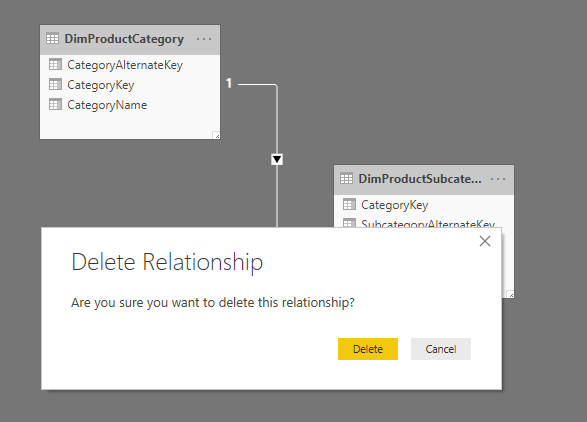
\includegraphics[width=13cm]{./Imagenes/Captura2-3} 
	\end{center}
\end{itemize} 

\begin{itemize}
	\item Creando la relacion entre la columna ProductSubcategoryKey a la columna SubcategoryKey en la tabla DimProductSubcategory, para crear una relación de Muchos a Uno (Many to One (*:1)), y una dirección de filtro cruzado (Cross filter direction) en ambos.
	\begin{center}
	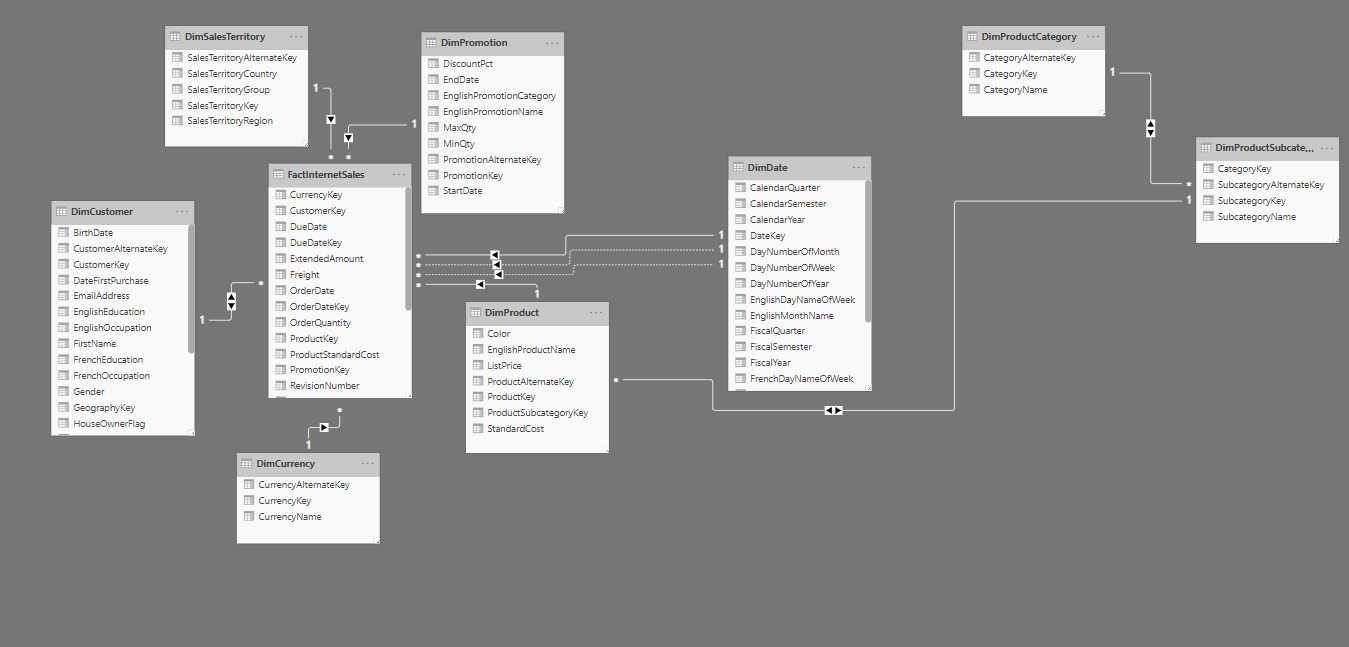
\includegraphics[width=13cm]{./Imagenes/Captura2-4} 
	\end{center}
\end{itemize} 


\textbf{Ejercicio 3: Cálculos}


\begin{itemize}
	\item Vista Data.
	\begin{center}
	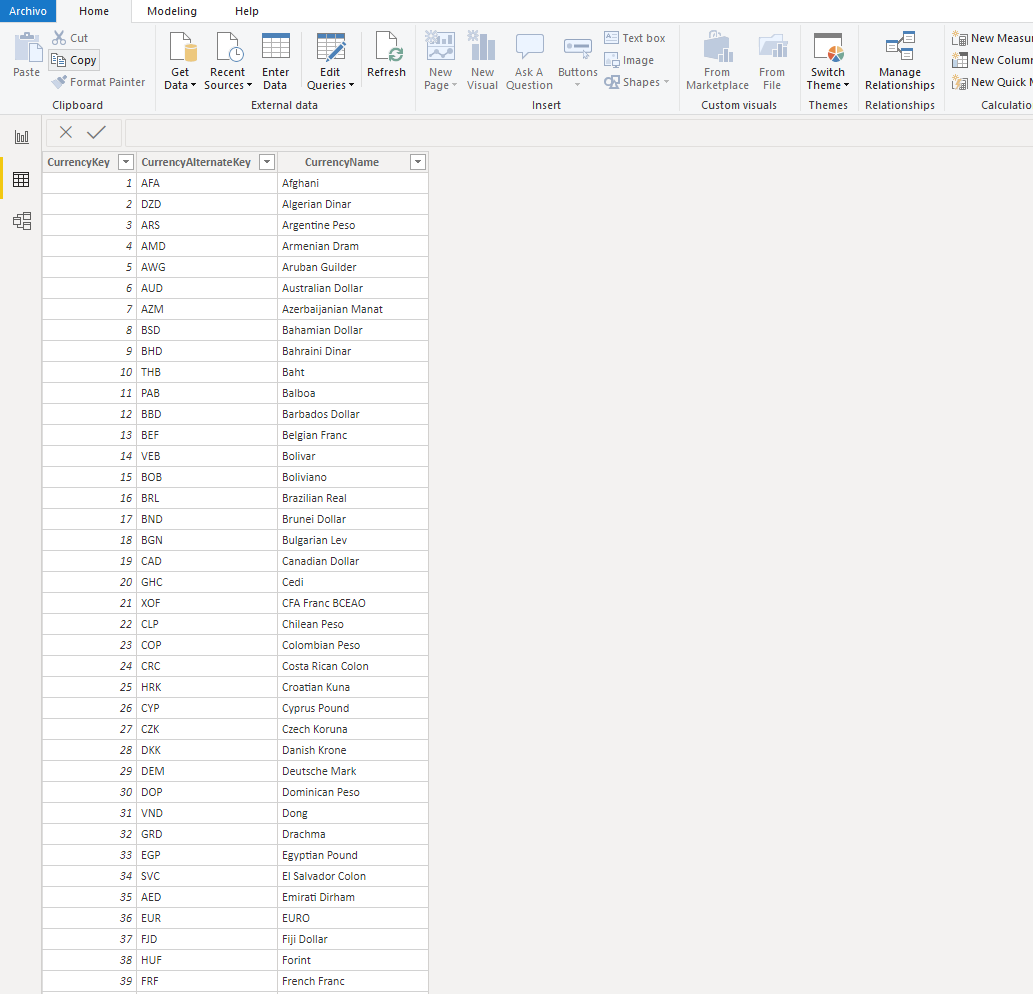
\includegraphics[width=13cm]{./Imagenes/Captura3-1} 
	\end{center}
\end{itemize} 

\begin{itemize}
	\item Vista Data de DimCustomer.
	\begin{center}
	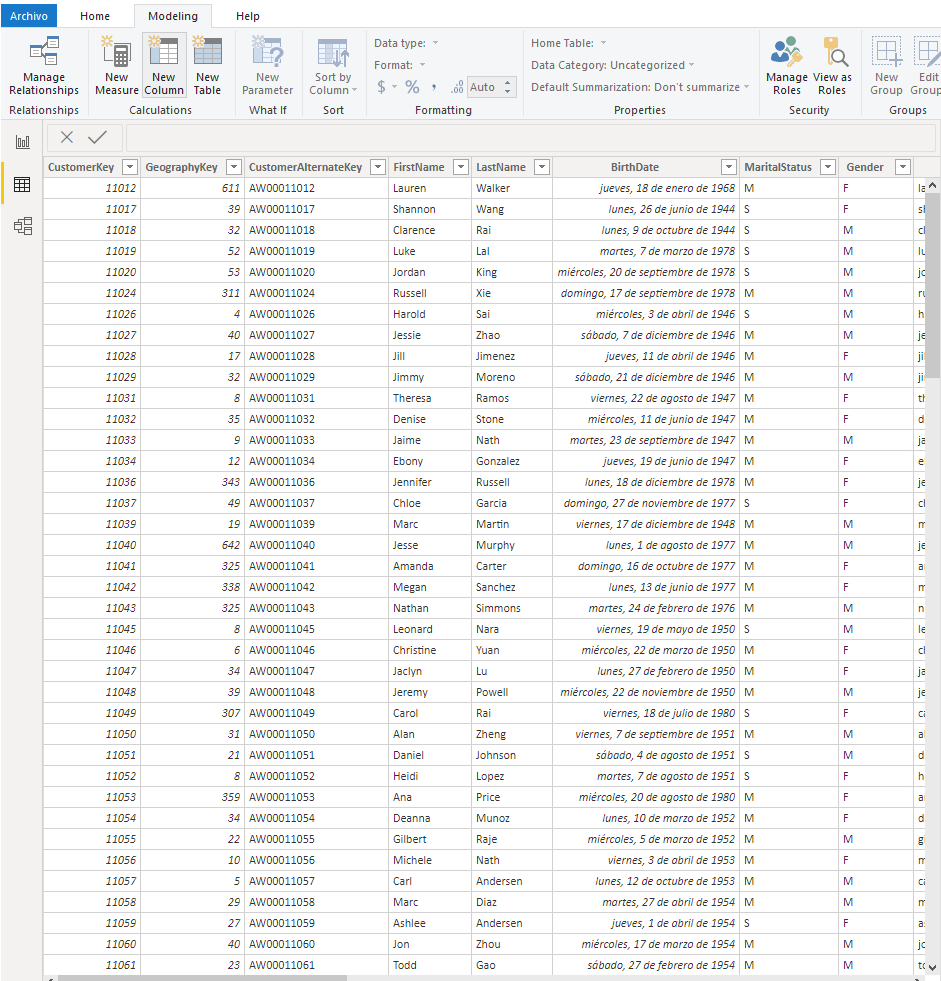
\includegraphics[width=13cm]{./Imagenes/Captura3-2} 
	\end{center}
\end{itemize} 

\begin{itemize}
	\item Nuevas columnas creadas, IncomeStatus, DaysSinceFirstPurchase, FullName, MaleFemale, Relationship.
	\begin{center}
	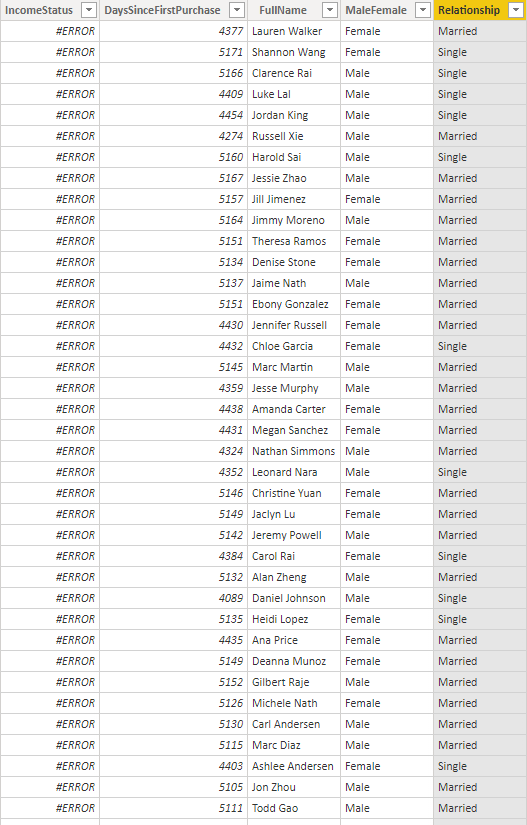
\includegraphics[width=10cm]{./Imagenes/Captura3-3} 
	\end{center}
\end{itemize} 

\begin{itemize}
	\item creando la columna MainCategory.
	\begin{center}
	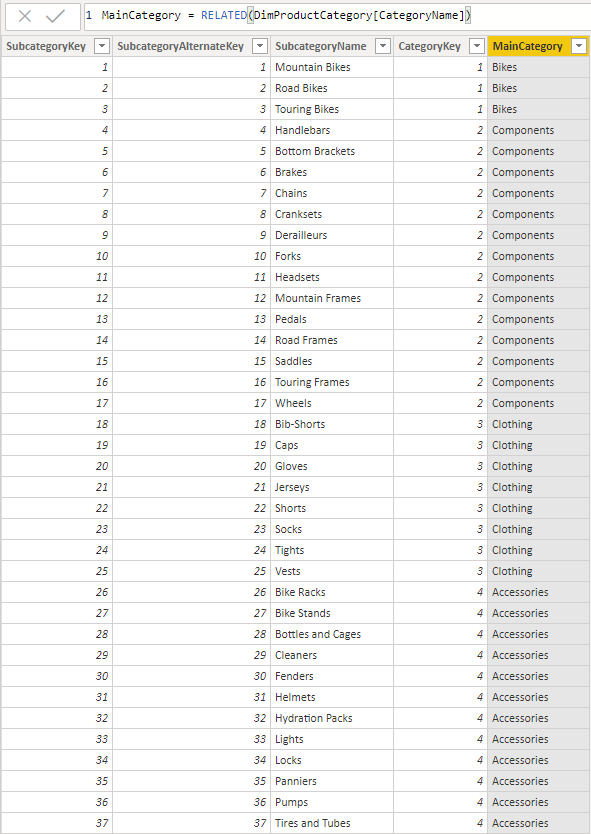
\includegraphics[width=10cm]{./Imagenes/Captura3-4} 
	\end{center}
\end{itemize}

\begin{itemize}
	\item creando la columna PromotionLengthDays.
	\begin{center}
	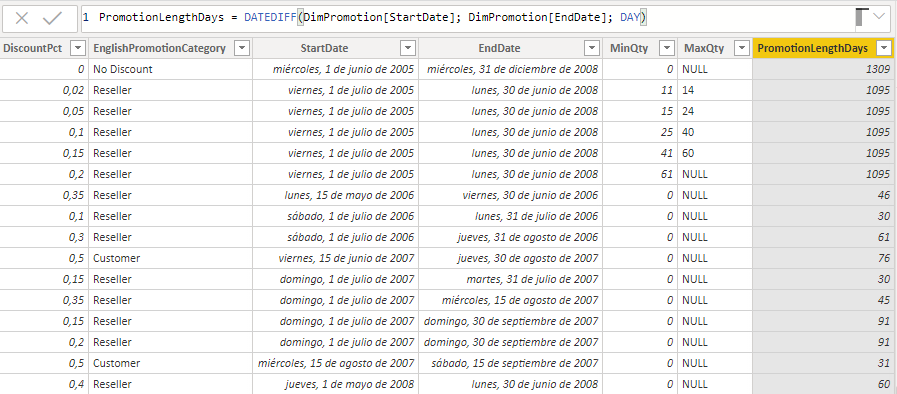
\includegraphics[width=10cm]{./Imagenes/Captura3-5} 
	\end{center}
\end{itemize}

\begin{itemize}
	\item creando la columna Profit.
	\begin{center}
	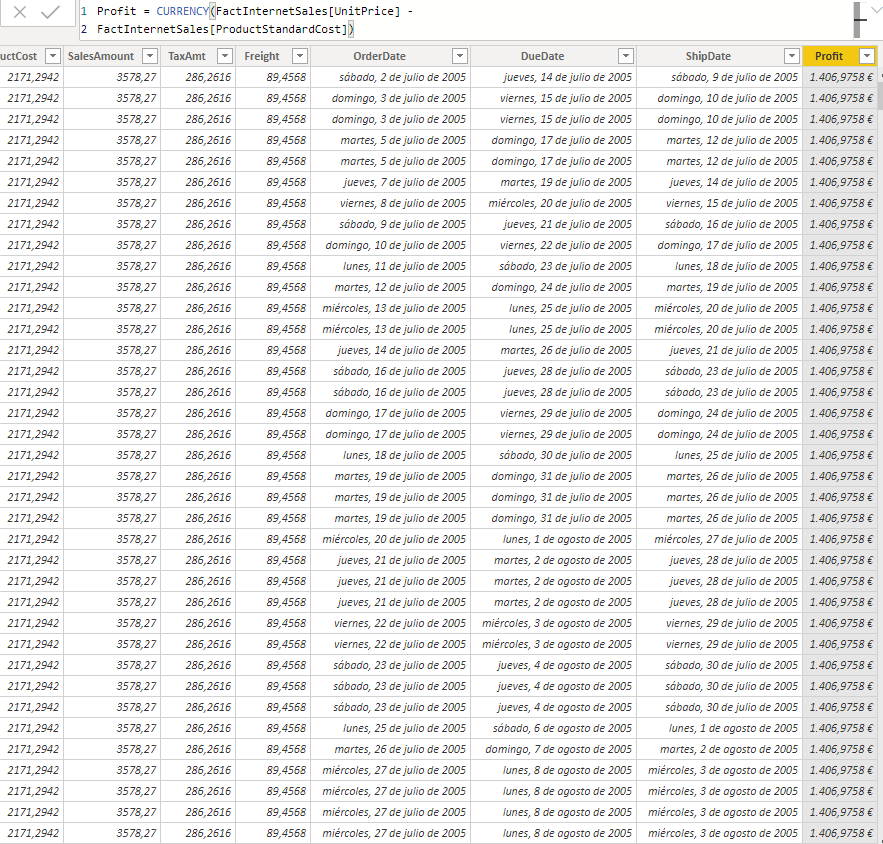
\includegraphics[width=10cm]{./Imagenes/Captura3-6} 
	\end{center}
\end{itemize}








